\def\detectionbranch{
    Nhánh xác định đối tượng\index{nhánh xác định đối tượng} của RetinaFocus được xây dựng dựa trên mô hình RetinaFace \cite{deng2020retinaface}, một mô hình một pha\index{một pha} giải quyết bài toán nhận diện khuôn mặt và đạt kết quả tốt trên bộ dữ liệu WIDER FACE \cite{yang2016wider}. \\

    \noindent
    \textbf{\textit{Giới thiệu chung về mô hình RetinaFace nguyên bản}} \\
    Mô hình RetinaFace \cite{deng2020retinaface} nguyên bản đạt độ chính xác lần lượt là 96.9\%, 96.1\% và 91.8\% trên bộ dữ liệu WIDER FACE val easy, medium và hard.
    Trong khi đó, với bộ dữ liệu WIDER FACE test, Mô hình RetinaFace \cite{deng2020retinaface} nguyên bản đạt độ chính xác lần lượt là 96.3\%, 95.6\% và 91.4\% tương ứng với bộ easy, medium và hard.

    \begin{figure}[H]
        \centering
        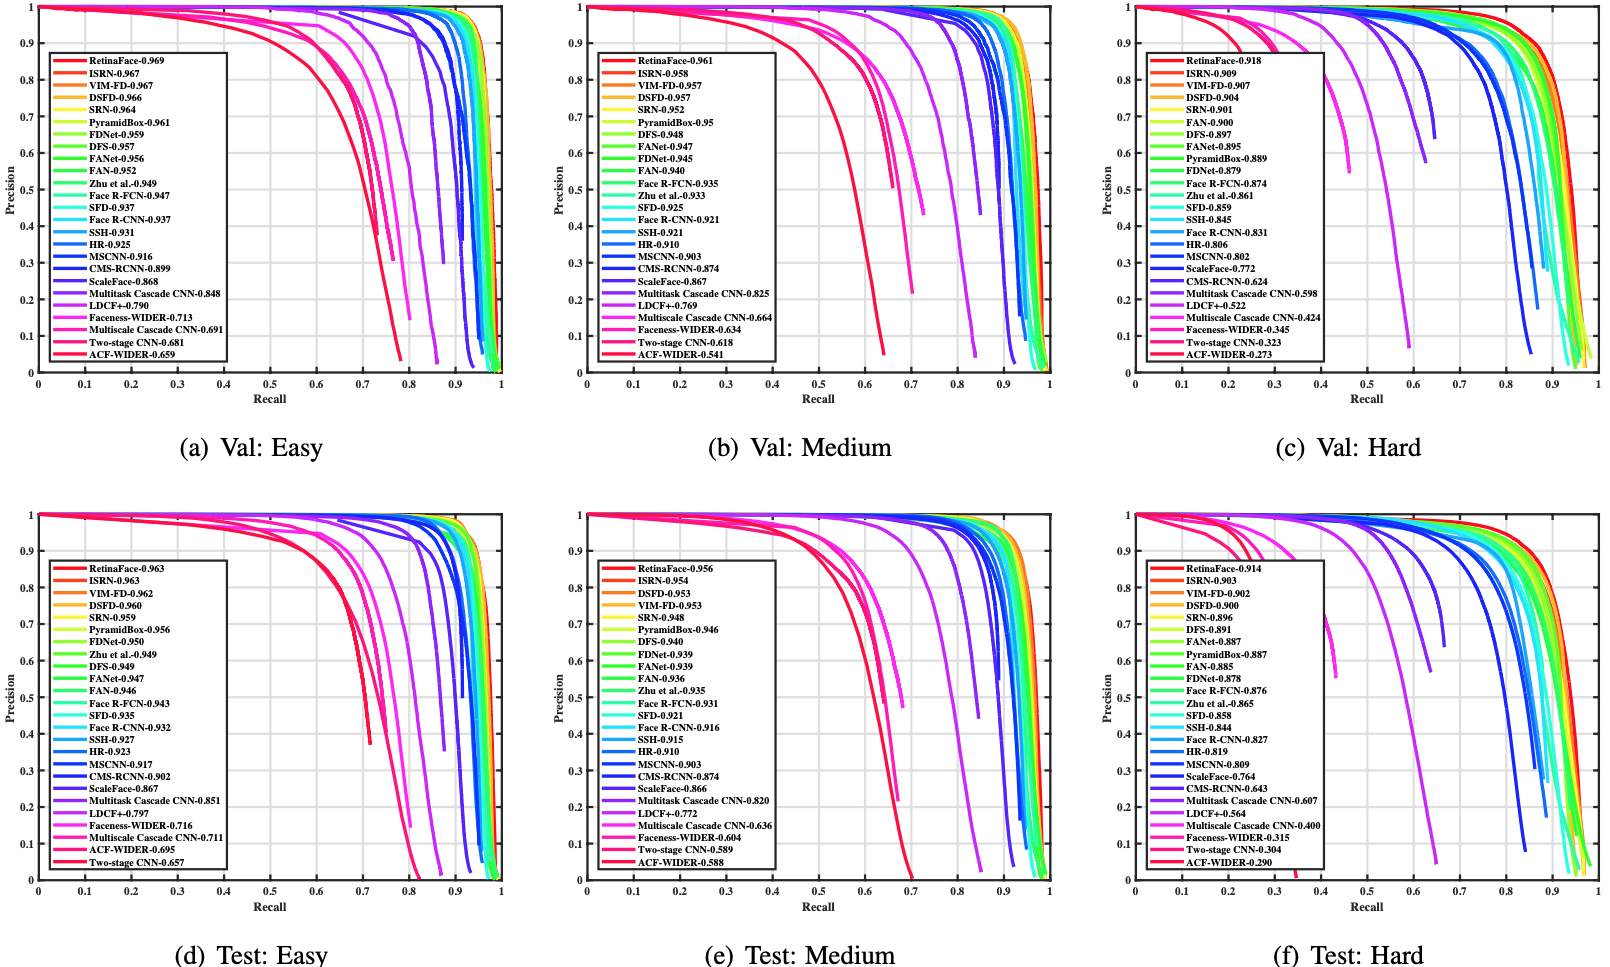
\includegraphics[width=15cm] {images/retinaface_results_3}
        \caption{Kết quả của mô hình RetinaFace nguyên bản trên bộ dữ liệu WIDER FACE val và test. (Nguồn: \cite{deng2020retinaface})}
        \label{fig:retinaface_results_3}
    \end{figure}

    \noindent
    Khi sử dụng kết quả nhận diện khuôn mặt làm đầu vào cho mô hình ArcFace \cite{deng2019arcface}, mô hình RetinaFace \cite{deng2020retinaface} nguyên bản không những đạt kết quả tốt trên bài toán nhận diện khuôn mặt mà nó còn giúp giúp cải thiện kết quả của bài toán nhận diện danh tính khuôn mặt\index{nhận diện danh tính khuôn mặt} khi so sánh với mô hình MTCNN \cite{zhang2016joint}.
    
    \noindent
    Việc sử dụng kiến trúc mô hình RetinaFace \cite{deng2020retinaface} nguyên bản cho nhánh xác định đối tượng\index{nhánh xác định đối tượng} giúp mô hình RetinaFocus tận dụng được kết quả tốt có sẵn trên bài toán nhận diện khuôn mặt.
    Và sau đó, mô hình RetinaFocus giúp cải thiện điểm yếu của mô hình RetinaFace khi xử lý với ảnh chất lượng cao thông qua nhánh tập trung đối tượng\index{nhánh tập trung đối tượng}.

    \begin{figure}[H]
        \centering
        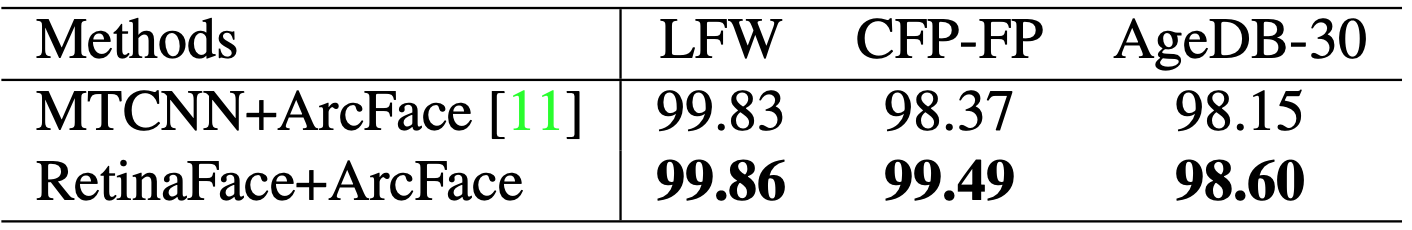
\includegraphics[width=10cm] {images/retinaface_results_2}
        \caption{Mô hình RetinaFace nguyên bản giúp cải thiện kết quả của bài toán nhận diện danh tính khuôn mặt\index{nhận diện danh tính khuôn mặt}. (Nguồn: \cite{deng2020retinaface})}
        \label{fig:retinaface_results_2}
    \end{figure}

    \noindent
    \textbf{\textit{Chi tiết kiến trúc của nhánh xác định đối tượng}} \\
    Nhánh xác định đối tượng\index{nhánh xác định đối tượng} cũng sử dụng kiến trúc FPN nhằm trích xuất đặc trưng của ảnh đầu vào với nhiều kích thước bản đồ đặc trưng\index{bản đồ đặc trưng} khác nhau.
    Hơn nữa, tương tự như RetinaFace \cite{deng2020retinaface}, nhánh xác định đối tượng\index{nhánh xác định đối tượng} đưa các bản đồ đặc trưng\index{bản đồ đặc trưng} này qua các Context Module \cite{najibi2017ssh} nhằm thu thập thêm các thông tin về background\index{background} xung quanh trước khi đưa ra dự đoán về hộp giới hạn\index{hộp giới hạn} chứa khuôn mặt.
    Ý tưởng sử dụng các khối Context Module \cite{najibi2017ssh} tỏ ra khá hiệu quả khi áp dụng với bài toán nhận diện khuôn mặt.

    \begin{figure}[H]
        \centering
        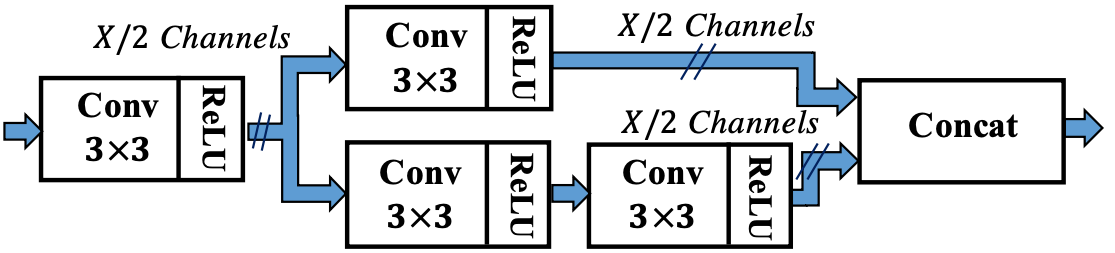
\includegraphics[width=10cm] {images/retinaface_context_module}
        \caption{Chi tiết kiến trúc nguyên bản của khối Context Module (Nguồn: \cite{najibi2017ssh})}
        \label{fig:retinaface_context_module}
    \end{figure}

    \noindent
    Đặc biệt trong việc định vị các mặt nhỏ, vì khi những thông tin về background\index{background} xung quanh như thân người sẽ có vai trò quan trọng giúp mô hình học tốt hơn.
    Trong kiến trúc của nhánh xác định đối tượng\index{nhánh xác định đối tượng}, ba bản đồ đặc trưng\index{bản đồ đặc trưng} \textit{{${P}_{3}, {P}_{4}, {P}_{5}$}} của FPN của mô hình xương sống được đưa qua ba khối Context Module độc lập.
    Mỗi khối Context Module gồm ba khối Conv nối tiếp nhau, nhưng bản đồ đặc trưng\index{bản đồ đặc trưng} đầu ra của mỗi khối Conv đều được concat lại với nhau để tạo ra bản đồ đặc trưng\index{bản đồ đặc trưng} cuối cùng của cả khối Context Module. \\

    \begin{figure}[H]
        \centering
        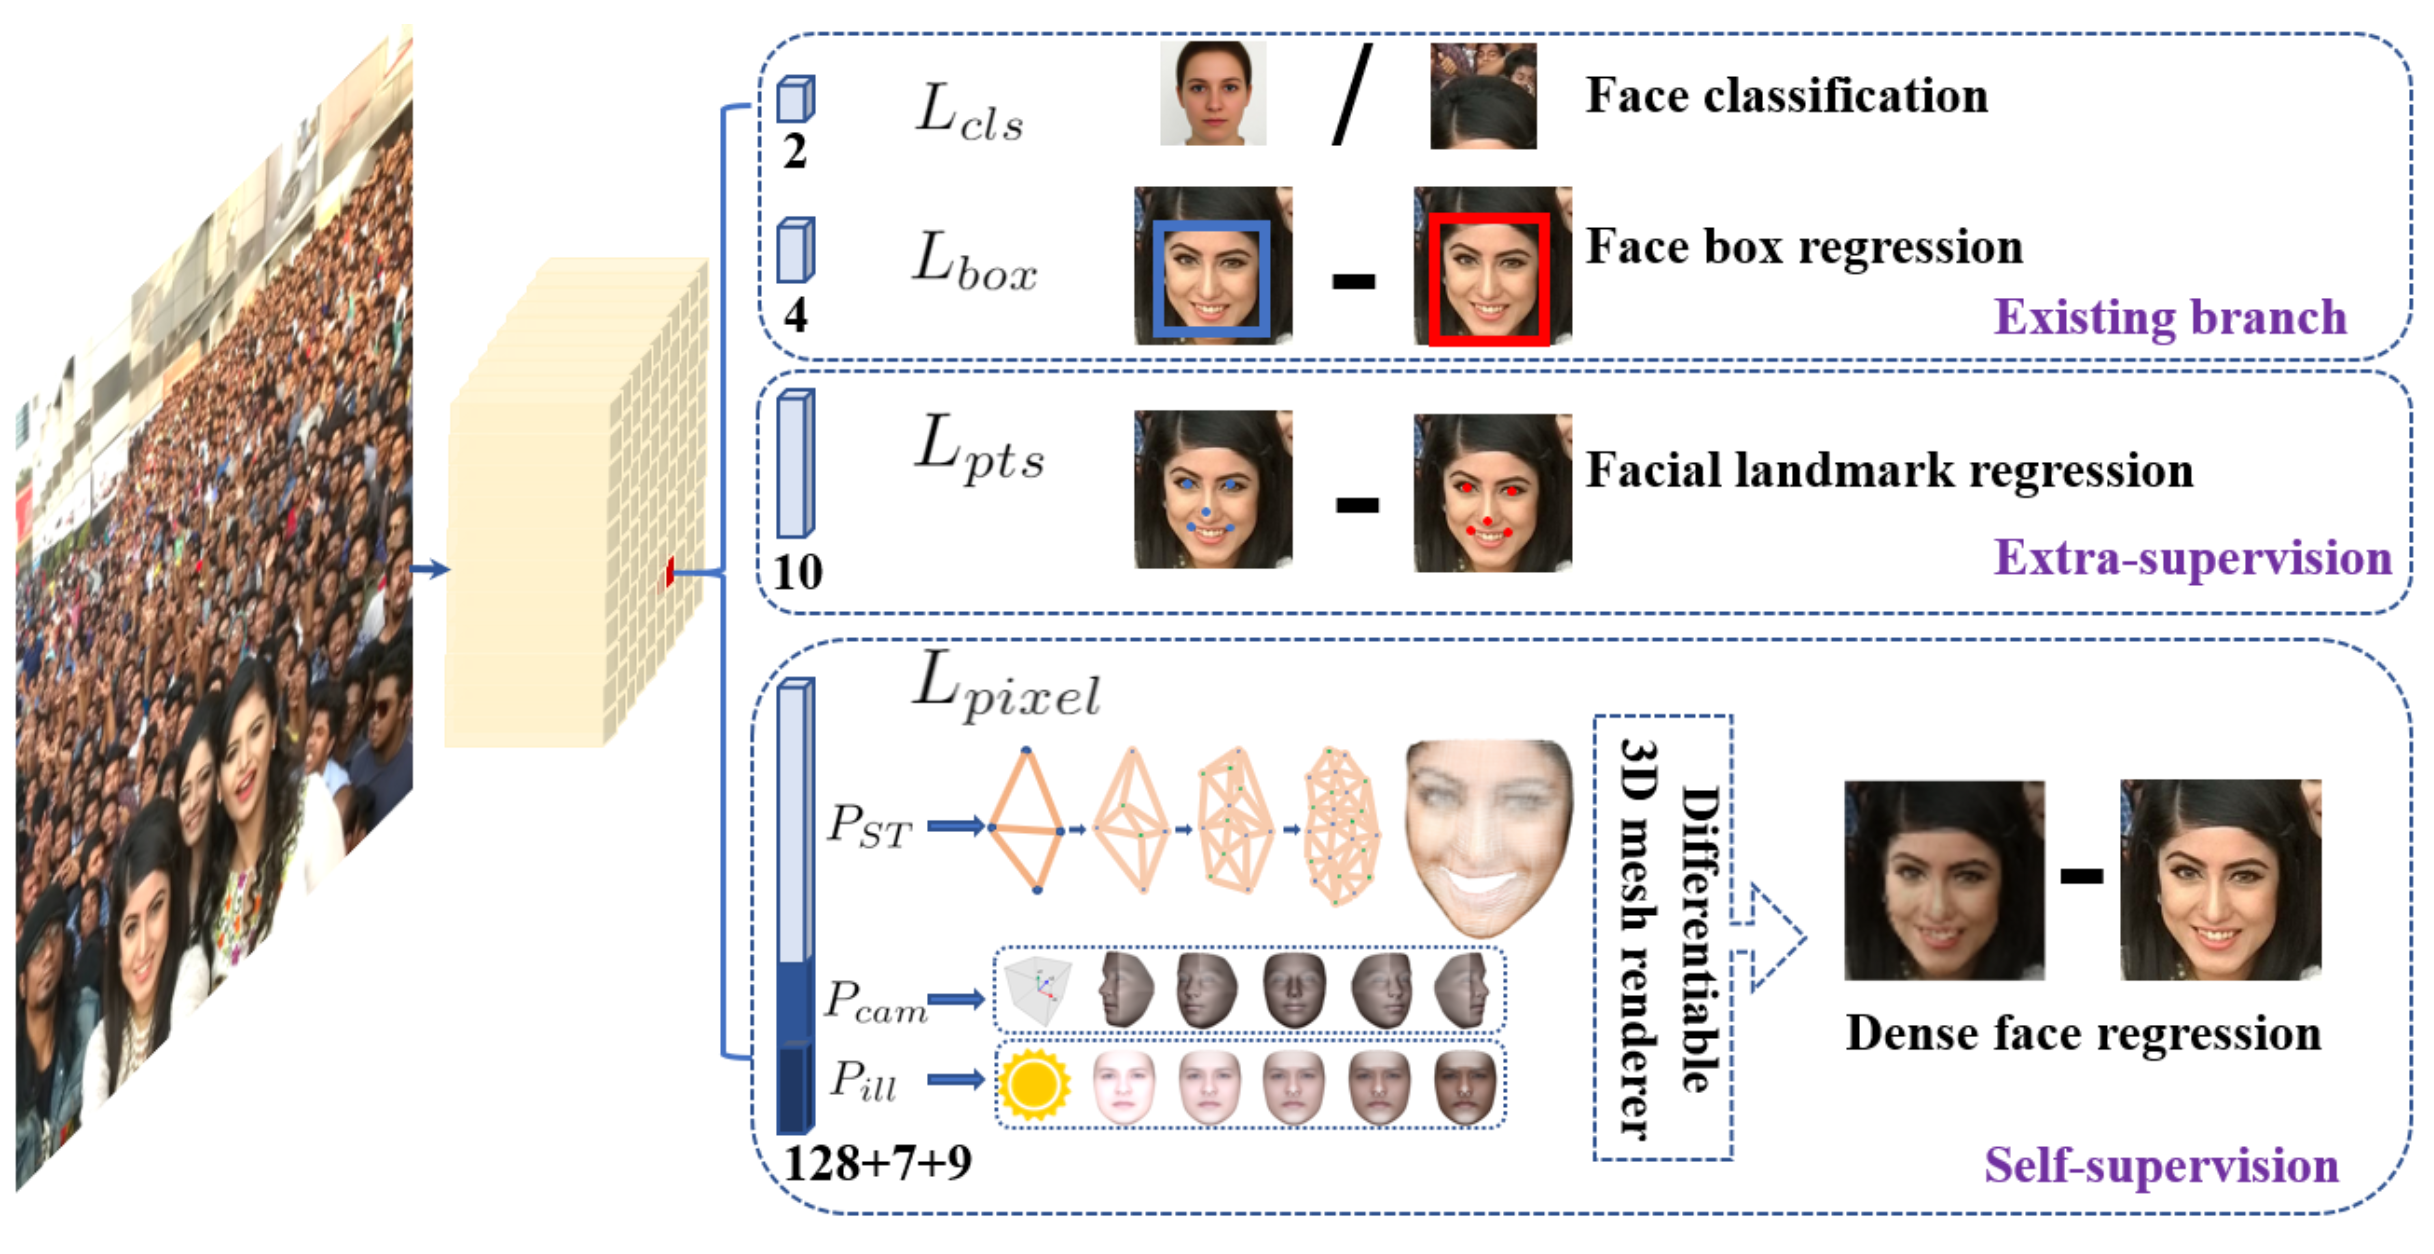
\includegraphics[width=10cm] {images/retinaface_loss_funcs}
        \caption{Ý tưởng các hàm mất mát đa nhiệm vụ\index{hàm mất mát đa nhiệm vụ} của mô hình RetinaFace. Ngoài hàm mất mát học tự giám sát\index{hàm mất mát học tự giám sát} \cite{zhou2019dense, genova2018unsupervised}, các hàm mất mát còn lại được kế thừa cho mô hình RetinaFocus (Nguồn: \cite{deng2020retinaface})}
        \label{fig:retinaface_loss_funcs}
    \end{figure}

    \noindent
    \textbf{\textit{Hàm mất mát đa nhiệm vụ}} \\
    Đầu ra nhánh xác định đối tượng\index{nhánh xác định đối tượng} của RetinaFocus gồm toạ độ của hộp giới hạn\index{hộp giới hạn} dự đoán của mô hình, toạ độ của landmarks của khuôn mặt và xác suất mà hộp giới hạn\index{hộp giới hạn} dự đoán đó chứa khuôn mặt.
    Các đầu ra này tiếp tục được đưa vào hàm mất mát đa nhiệm vụ\index{hàm mất mát đa nhiệm vụ}, tương tự như mô hình RetinaFace \cite{deng2020retinaface}. \\
    Cụ thể, trong quá trình huấn luyện mô hình, với mỗi khu vực mỏ neo\index{khu vực mỏ neo}, nhánh xác định đối tượng\index{nhánh xác định đối tượng} của mô hình RetinaFocus tối ưu hàm mất mát đa nhiệm vụ\index{hàm mất mát đa nhiệm vụ} dưới đây:

    \begin{equation}
        \begin{split}
        L  & =  L_{cls}(p_i, p^{*}_i) + \lambda_1 p^{*}_i L_{box}(t_i, t^{*}_i) + \lambda_2 p^{*}_i L_{pts} (l_i, l^{*}_i).\\
        \end{split}
        \label{eq:retinaface_loss}
    \end{equation}

    \noindent
    trong đó: \\
    - Các trọng số $\lambda_1, \lambda_2$ được cấu hình mặc định theo mô hình RetinaFace \cite{deng2020retinaface} lần lượt là 0.25, 0.1 và 0.01. Các trọng số này đóng vai trò giúp cân bằng tỷ lệ của các thành phần $L_{cls}$, $L_{box}$ và $L_{pts}$ của hàm mất mát đa nhiệm vụ\index{hàm mất mát đa nhiệm vụ}. \\
    - Hàm mất mát phân lớp mặt: \\
    $L_{cls}(p_i, p^{*}_i)$ với $p_i$ là xác suất mà mô hình dự đoán một khu vực mỏ neo\index{khu vực mỏ neo} có chứa là khuôn mặt hay không.
    Ta có $p^{*}_i = 1$ nếu khu vực mỏ neo\index{khu vực mỏ neo} đó chứa khuôn mặt còn $p^{*}_i = 0$ nếu khu vực mỏ neo\index{khu vực mỏ neo} đó không chứa khuôn là mặt. \\
    - Hàm mất mát hồi quy định vị vị trí của hộp giới hạn\index{hộp giới hạn}: \\
    $L_{box}(t_i, t^{*}_i)$ với $t_i=\{t_x, t_y, t_w, t_h\}_i$ và $t^{*}_i=\{t^{*}_x, t^{*}_y, t^{*}_w, t^{*}_h\}_i$ lần lượt là bộ bốn tham số đại diện cho toạ độ của khu vực mỏ neo\index{khu vực mỏ neo} mà mô hình dự đoán là mặt và hộp giới hạn\index{hộp giới hạn} groundtruth\index{groundtruth} từ bộ dữ liệu.
    (x là toạ độ x của điểm góc trái trên, y là toạ độ y của điểm góc trái trên, w là chiều rộng của hộp giới hạn\index{hộp giới hạn} và h là chiều cao của hộp giới hạn\index{hộp giới hạn}). \\
    - Hàm mất mát hồi quy định vị vị trí của landmarks: \\
    $L_{pts} (l_i, l^{*}_i)$ với $l_i=\{l_{x_1}, l_{y_1}, \dots , l_{x_5}, l_{y_5}\}_i$ và $l^{*}_i=\{l^{*}_{x_1}, l^{*}_{y_1}, \dots , l^{*}_{x_5}, l^{*}_{y_5}\}_i$ lần lượt là bộ mười tham số đại diện cho toạ độ của năm landmarks mà mô hình dự đoán ứng với mỗi hộp giới hạn\index{hộp giới hạn} dự đoán và năm groundtruth\index{groundtruth} landmarks của mỗi groundtruth\index{groundtruth} hộp giới hạn\index{hộp giới hạn} từ bộ dữ liệu. \\

    \noindent
    \textbf{\textit{So sánh giữa mô hình RetinaFace nguyên bản và nhánh xác định đối tượng của mô hình RetinaFocus}} \\
    Mặc dù kế thừa kiến trúc mô hình RetinaFace nguyên bản để xây dựng nhánh xác định đối tượng của mô hình RetinaFocus, tuy nhiên, vẫn có những sự khác biệt nhất định.

    \begin{figure}[H]
        \centering
        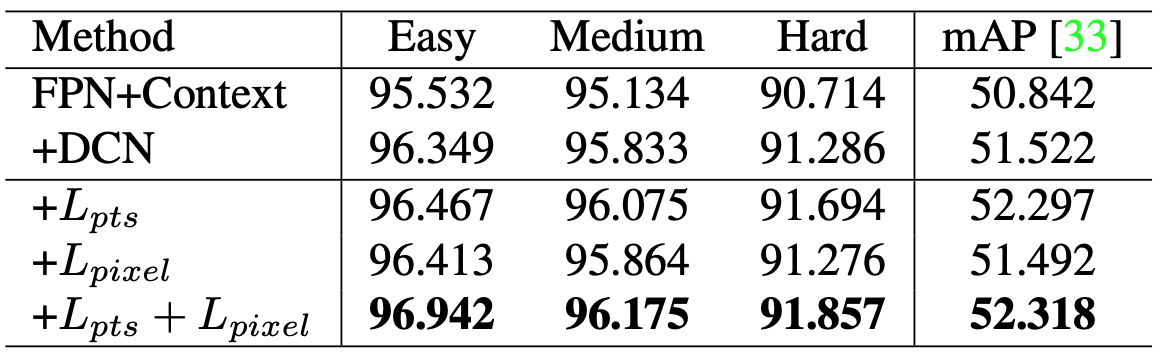
\includegraphics[width=10cm] {images/retinaface_results_1}
        \caption{Vai trò của lớp DCN và hàm mất mát học tự giám sát đối với kết quả của mô hình RetinaFace nguyên bản trên bộ dữ liệu WIDER FACE (Nguồn: \cite{deng2020retinaface})}
        \label{fig:retinaface_results_1}
    \end{figure}

    \noindent
    Đầu tiên, mô hình RetinaFace nguyên bản sử dụng các lớp Conv được kế thừa từ mô hình DCN \cite{dai2017deformable}, giúp nâng cao độ chính xác của mô hình hơn so với lớp Conv thông thường.
    Trong khi đó, nhánh xác định đối tượng của mô hình RetinaFocus không sử dụng lớp DCN này. \\
    Tiếp theo, mô hình RetinaFace bổ sung thêm các hàm mất mát học tự giám sát\index{hàm mất mát học tự giám sát} \cite{zhou2019dense, genova2018unsupervised} vào hàm mất mát đa nhiệm vụ\index{hàm mất mát đa nhiệm vụ} chung giúp cải thiện độ chính xác khi nhận diện khuôn mặt.
    Nhánh xác định đối tượng của mô hình RetinaFocus không sử dụng bổ trợ các hàm mất mát này. \\
    Cuối cùng, về mặt kiến trúc của mô hình RetinaFace nguyên bản sử dụng các bản đồ đặc trưng\index{bản đồ đặc trưng} $C_6, P_5, P_4, P_3$ và $P_2$ làm đầu vào cho các khối Context Module \cite{najibi2017ssh}.
    Trong khi đó, nhánh xác định đối tượng của mô hình RetinaFocus chỉ sử dụng các bản đồ đặc trưng\index{bản đồ đặc trưng} $P_5, P_4$ và $P_3$ làm đầu vào cho các khối Context Module \cite{najibi2017ssh}. \\
    Những sự khác biệt này được đưa ra dựa trên điều kiện trong quá trình lập trình cài đặt mô hình RetinaFocus.
}